

\begin{frame}{\ft{Overview of the 
			Software Development Market}}

%\doubleFrame{EC1.}

\pgfdeclareverticalshading{myshading}{100bp}{color(0bp)=(yellow!60); 
	%color(30bp)=(yellow!10); 
	%color(70bp)=(green!10); 
	color(100bp)=(green!10)}

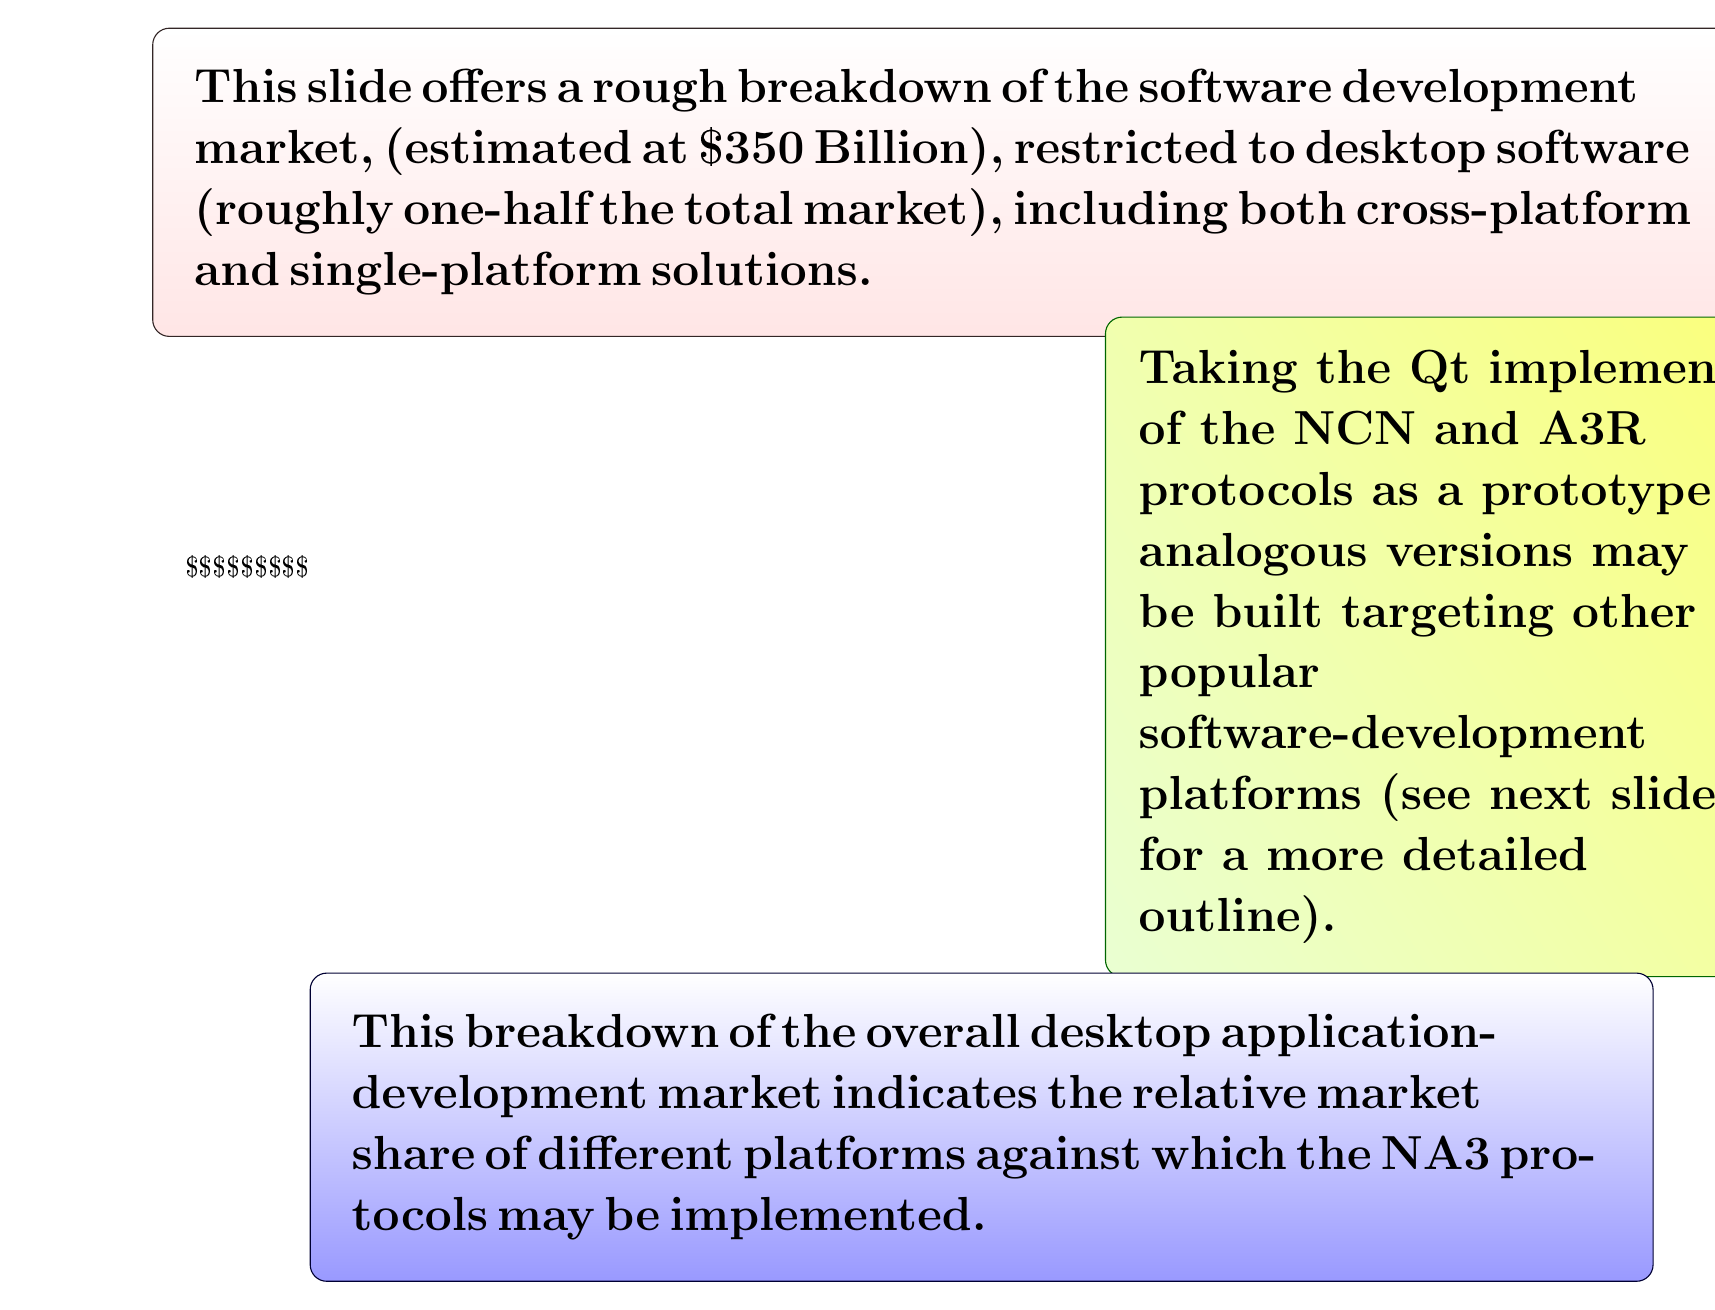
\begin{tikzpicture}


\pie [rotate = 180,
/tikz/nodes={text=white, font=\bfseries},
text=legend,radius = 7.5,%pos = {4,6},
%/tikz/every legend/.style={text=black},
color={
    lqboutercolor!30!purple,	
	{rgb:red,0;green,0.24;blue,0.25}, 	
	{rgb:red,0.2;green,0;blue,0.5},
    red!40!green,	
	{rgb:red,0.1;green,0.2;blue,0.2},},
polar, explode=0.2%, text=legend
]
{   15/Qt/(\$27b), 
	60/Windows MFC/(\$135 billion),
	12/Apple XCode/(\$25b), 
	7/Java/(\$13b), 
	6/Other/(\$10b)}
{"(\$27b)","(\$135 billion)","(\$25b)",
	"(\$13b)",""	
	};

 \node [anchor=west,inner sep=15, text width=20cm,
 draw = pink!20!black,
 top color=white,text=black,
 bottom color=pink!40,
 rounded corners=6pt%,
 %blur shadow={shadow blur steps=2}
 ]
 (longnote) at (-2,5) {\baselineskip=22pt%  %{\color{rb!85!red}{
 	{\LARGE \textbf{This slide offers a rough 
 breakdown of the software development market, 
 (estimated at \$350 Billion), restricted to 
 desktop software (roughly one-half the 
 total market), including both cross-platform 
 and single-platform solutions.}}\par};
%[/tikz/every legend entry/.style={text=red}]

 \node [anchor=west,inner sep=12, text width=7.8cm,
 draw=green!40!black,shading=myshading, 
 shading angle=125,align=flush left,
% left color=yellow!20,
% right color=green!10,
 text=black,rounded corners=6pt%,
 %blur shadow={shadow blur steps=2}
 ]
 (longnote) at (10.1,-.9) {\baselineskip=22pt%  %{\color{rb!85!red}{
 	{\LARGE \textbf{\makebox{Taking the 
 Qt implementations} of the NCN and A3R 
 protocols as a prototype, 
 analogous versions may be 
 built targeting other popular 
 software-development platforms 
 (see next slide for a more detailed outline).}}\par};


 \node [anchor=west,inner sep=15, text width=16cm,
 draw = blue!20!black,
 top color=white,text=black,
 bottom color=blue!40,
 rounded corners=6pt%,
 %blur shadow={shadow blur steps=2}
 ]
 (longnote) at (0,-7) {\baselineskip=22pt%  %{\color{rb!85!red}{
 	{\LARGE \textbf{This breakdown of 
the overall desktop application-development 
market indicates the relative market 
share of different platforms against which 
the NA3 protocols may be implemented.}}\par};
 
\end{tikzpicture}


\end{frame}

